\documentclass{report}
\usepackage[utf8]{inputenc}
\usepackage[a4paper, total={8in, 9in}]{geometry}
\usepackage{amsmath, amssymb}
\usepackage{bm}
\usepackage{graphicx}
\usepackage{subcaption}
\usepackage{caption}
\usepackage[colorlinks=true]{hyperref}

\title{Transition path sampling and the calculation of free energies: pnp}
\author{Schwartz group}
\begin{document}
\maketitle

\section{Choice of reactive trajectory}
\begin{figure}[ht!]
\centering
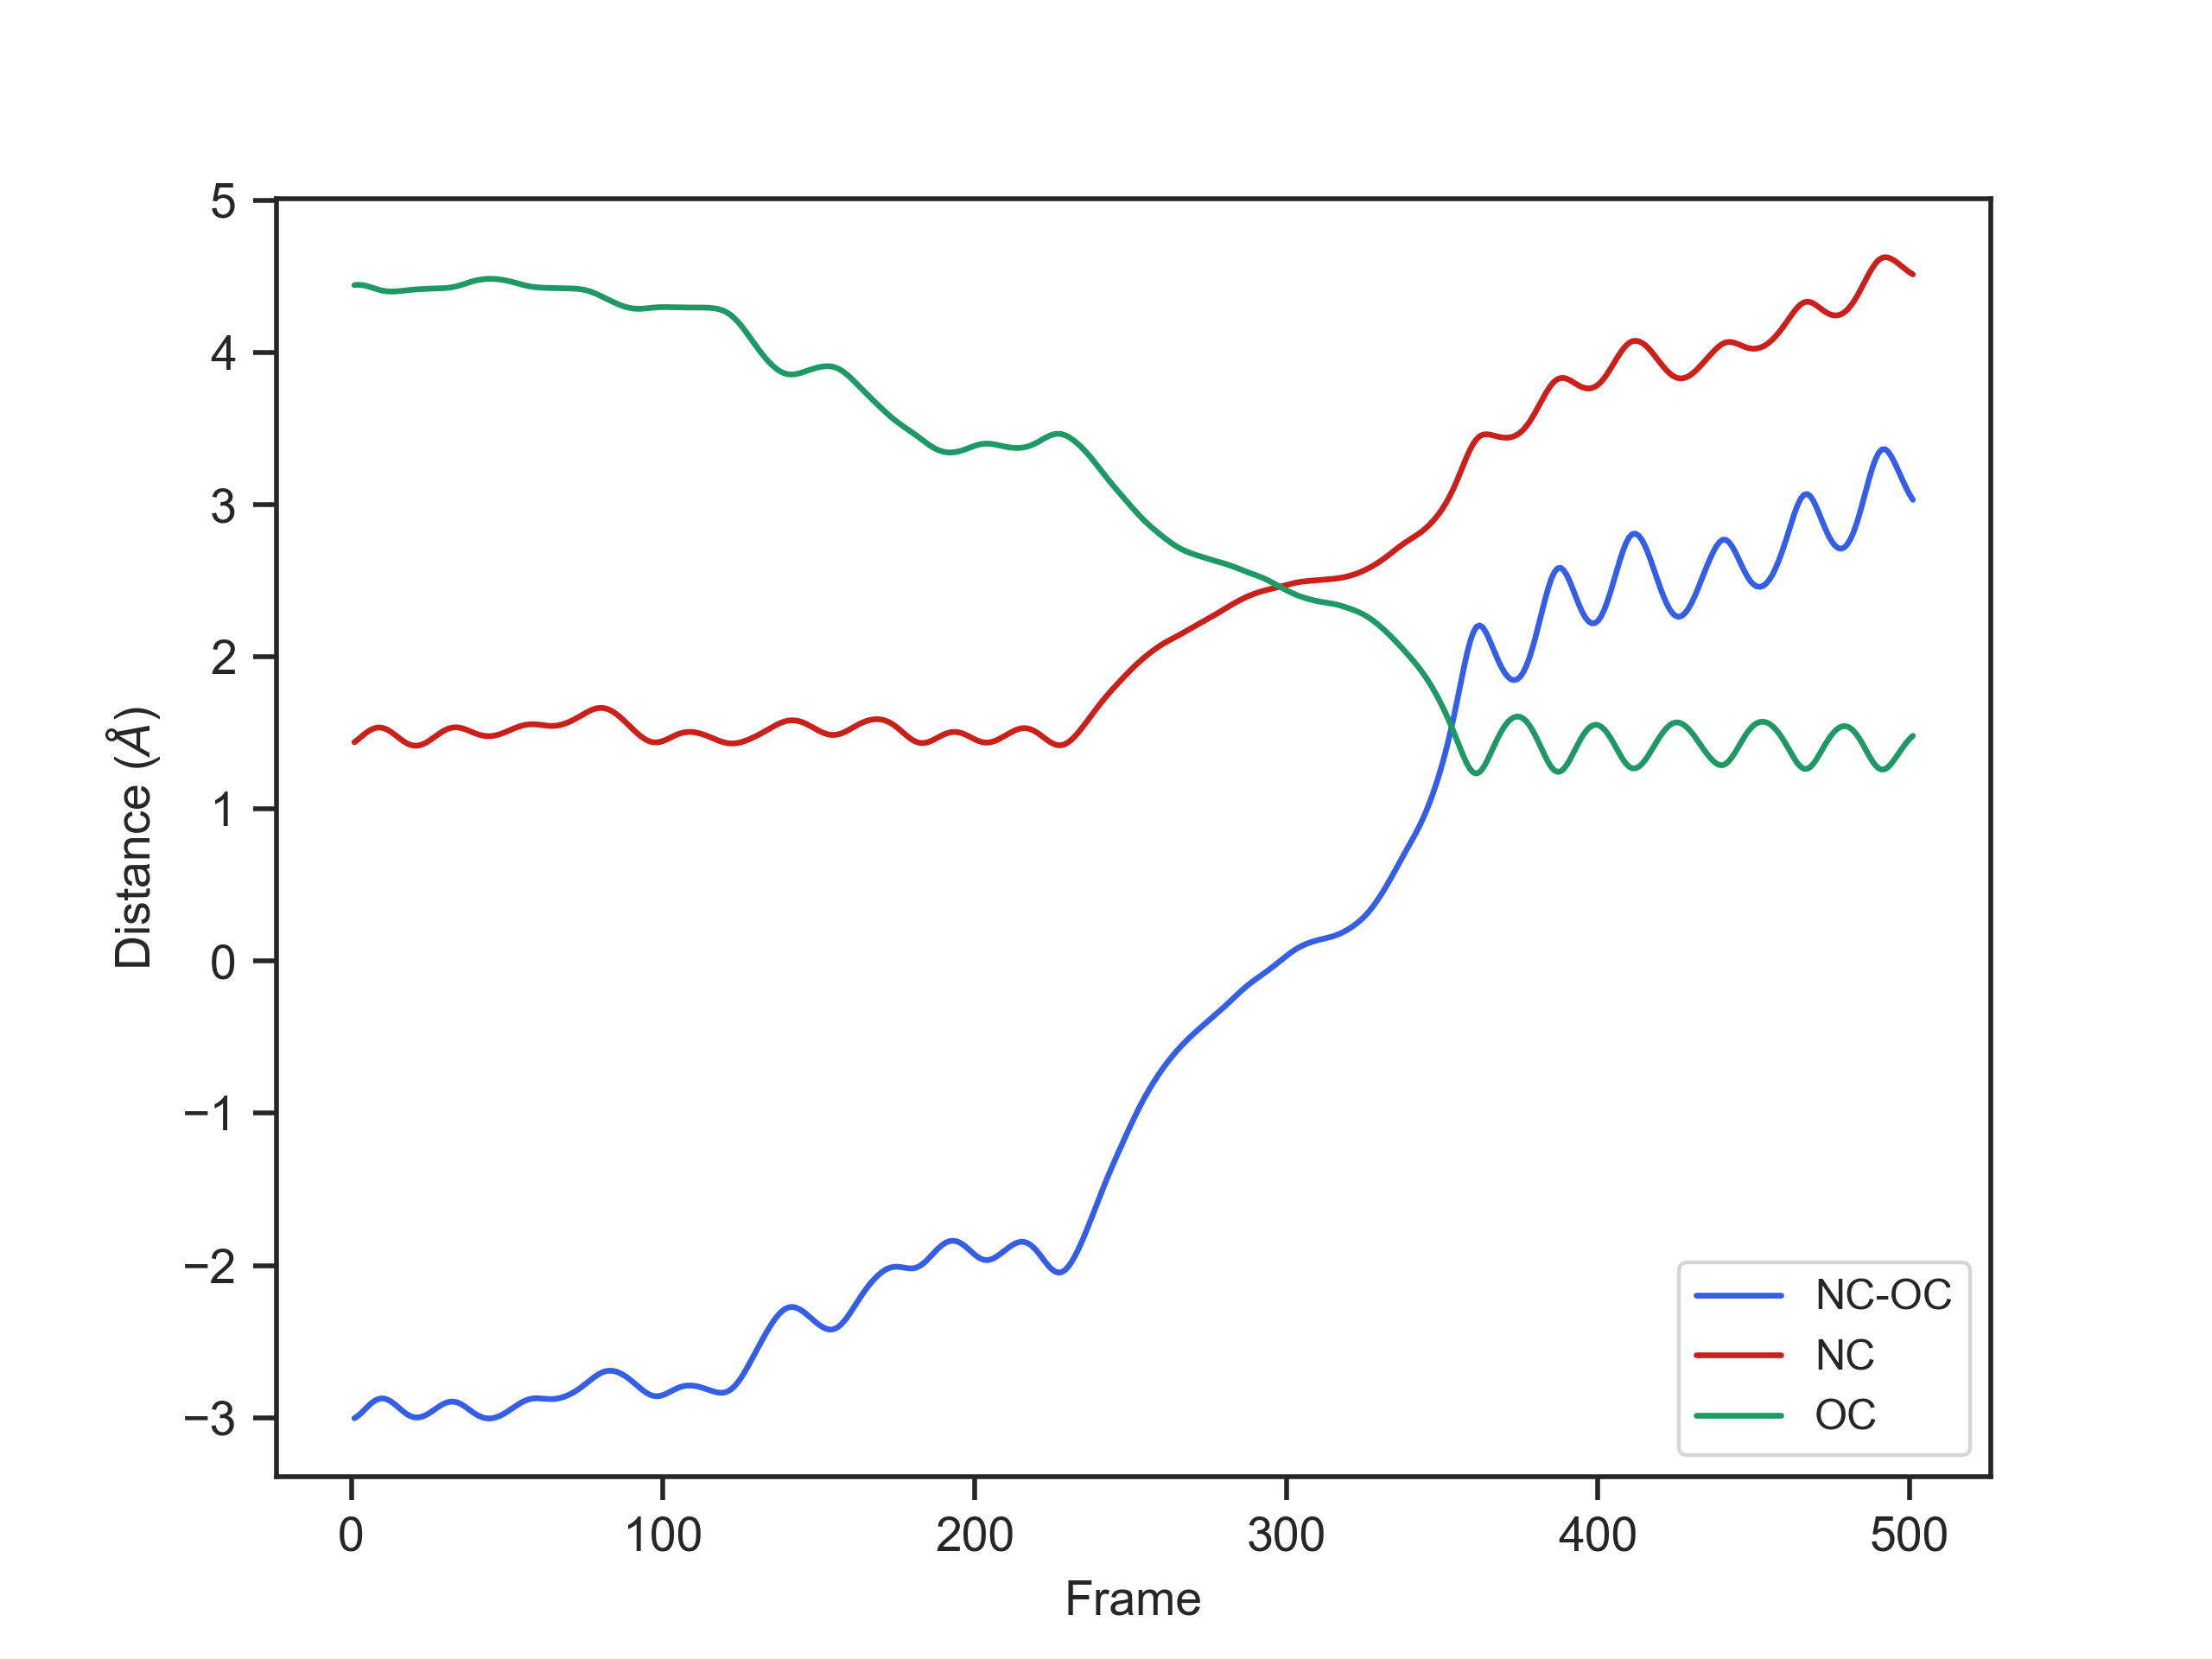
\includegraphics[scale=0.75]{figures/dis_nc-oc-90.png}
\caption{Variation of the order parameters as a function of time for a typical 
reactive trajectory for the reaction catalyzed by human purine nucleoside phosphorylase}
\label{fig:fig}
\end{figure}

\begin{center}
  \begin{tabular}{ l | c  }
    %\hline
    %Parameter & \\ 
    \hline
    Range & $\left[-3.04,3.04\right]$ {\AA}\\ 
    Number of windows & 30  \\ 
    Window size & $0.28$ {\AA} \\
    Overlap & 0.08 {\AA} \\
    \hline
  \end{tabular}
\end{center}

\begin{figure}[ht!]
\centering
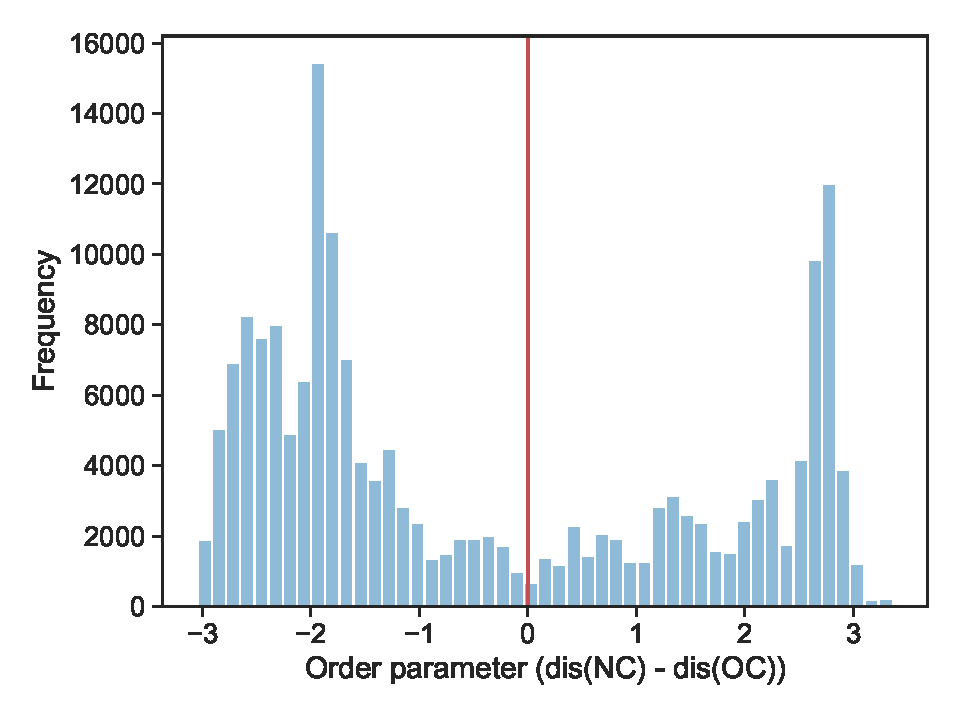
\includegraphics[scale=0.75]{figures/dist.pdf}
\caption{Frequency of the order parameter values observed using short TPS trajectories represented as histograms}
\end{figure}


\begin{figure}[ht!]
\centering
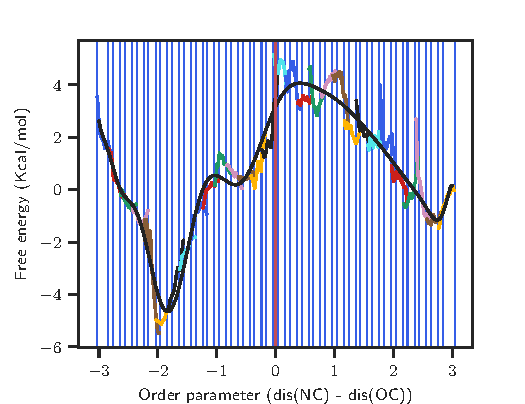
\includegraphics[scale=1.0]{figures/pnp-fenergy.pdf}
\caption{Free energy as a function of the order parameter for the reaction catalyzed by human purine nucleoside phosphorylase}
\end{figure}

\end{document}
